\documentclass[14pt, aspectratio=43]{beamer}
\usepackage[utf8]{inputenc}
\usepackage[english]{babel}
\usepackage{amsthm}
\usepackage{mathtools}
\usepackage{physics}
\usepackage{calligra}
\usepackage{csquotes}
\usepackage{tensor}
\usepackage[thicklines]{cancel}
\usepackage{tcolorbox}
\usepackage{pstricks}
\usepackage{bm}
\usepackage{systeme}
\usepackage{multicol}

\DeclareMathAlphabet{\mathcalligra}{T1}{calligra}{m}{n}
\DeclareFontShape{T1}{calligra}{m}{n}{<->s*[2.2]callig15}{}
\newcommand{\scriptr}{\mathcalligra{r}\,}
\newcommand{\boldscriptr}{\pmb{\mathcalligra{r}}\,}
\def\rc{\scriptr}
\def\brc{\boldscriptr}
\def\hrc{\hat\brc}
\newcommand{\ie}{\emph{i.e.}} %id est
\newcommand{\eg}{\emph{e.g.}} %exempli gratia
\newcommand{\rtd}[1]{\ensuremath{\left\lfloor #1 \right\rfloor}}
\newcommand{\dirac}[1]{\ensuremath{\delta \left( #1 \right)}}
\newcommand{\diract}[1]{\ensuremath{\delta^3 \left( #1 \right)}}
\newcommand{\e}{\ensuremath{\epsilon_0}}
\newcommand{\m}{\ensuremath{\mu_0}}
\newcommand{\V}{\ensuremath{\mathcal{V}}}
\newcommand{\prnt}[1]{\ensuremath{\left(#1\right)}} %parentheses
\newcommand{\colch}[1]{\ensuremath{\left[#1\right]}} %square brackets
\newcommand{\chave}[1]{\ensuremath{\left\{#1\right\}}}  %curly brackets

\useoutertheme{infolines}
\useinnertheme{rectangles}
\usefonttheme{professionalfonts}


\definecolor{orange}{HTML}{f28165}
\definecolor{gray}{HTML}{303030}
\definecolor{yellow}{HTML}{f0be52}
\definecolor{lightorange}{HTML}{f19e58}

\renewcommand{\CancelColor}{\color{orange}}

\makeatletter
\newcommand{\mybox}[1]{%
  \setbox0=\hbox{#1}%
  \setlength{\@tempdima}{\dimexpr\wd0+13pt}%
  \begin{tcolorbox}[colback=orange,colframe=orange,boxrule=0.5pt,arc=4pt,
      left=6pt,right=6pt,top=6pt,bottom=6pt,boxsep=0pt,width=\@tempdima]
    \textcolor{white}{#1}
  \end{tcolorbox}
}
\makeatother

\usecolortheme[named=orange]{structure}
\usecolortheme{sidebartab}
\usecolortheme{orchid}
\usecolortheme{whale}
\setbeamercolor{alerted text}{fg=yellow}
\setbeamercolor{block title alerted}{bg=alerted text.fg!90!black}
\setbeamercolor{block title example}{bg=lightorange!60!black}
\setbeamercolor{background canvas}{bg=gray}
\setbeamercolor{normal text}{bg=gray,fg=white}

\setbeamertemplate{footline}
        {
      \leavevmode%
      \hbox{%
      \begin{beamercolorbox}[wd=.333333\paperwidth,ht=2.25ex,dp=1ex,center]{author in head/foot}%
        \usebeamerfont{author in head/foot}\insertshortauthor~~(\insertshortinstitute)
      \end{beamercolorbox}%
      \begin{beamercolorbox}[wd=.333333\paperwidth,ht=2.25ex,dp=1ex,center]{title in head/foot}%
        \usebeamerfont{title in head/foot}\insertshorttitle
      \end{beamercolorbox}%
      \begin{beamercolorbox}[wd=.333333\paperwidth,ht=2.25ex,dp=1ex,center]{date in head/foot}%
        \usebeamerfont{date in head/foot}\insertshortdate{}%\hspace*{2em}

    %#turning the next line into a comment, erases the frame numbers
        %\insertframenumber{} / \inserttotalframenumber\hspace*{2ex} 

      \end{beamercolorbox}}%
      \vskip0pt%
    }


\setbeamertemplate{blocks}[rectangle]
\setbeamercovered{dynamic}

\setbeamertemplate{section page}
{
	\begin{centering}
		\begin{beamercolorbox}[sep=27pt,center]{part title}
			\usebeamerfont{section title}\insertsection\par
			\usebeamerfont{subsection title}\insertsubsection\par
		\end{beamercolorbox}
	\end{centering}
}

%\setbeamertemplate{subsection page}
%{
%	\begin{centering}
%		\begin{beamercolorbox}[sep=12pt,center]{part title}
%			\usebeamerfont{subsection title}\insertsubsection\par
%		\end{beamercolorbox}
%	\end{centering}
%}

\newcommand{\hlight}[1]{\colorbox{violet!50}{#1}}
\newcommand{\hlighta}[1]{\colorbox{red!50}{#1}}
\usepackage{tikz}
\usepackage{pgfplots}
\newcommand{\x}{\boldsymbol{x}}
\renewcommand{\a}{\boldsymbol{a}}
\renewcommand{\b}{\boldsymbol{b}}
\renewcommand{\c}{\boldsymbol{c}}
\newcommand{\R}{\mathbb{R}}
\title{Calculus Objectives Presentation}
\subtitle{Intersections of vectors and vector-valued equations}
\author[Anish \& Zachary]{Anish Goyal \and Zachary Cobb}
\institute[GSMST]{
    Gwinnett School of Math,%
    \\%
     Science, and Technology%
} %You can change the Institution if you are from somewhere else
\date{March 30, 2023}
\titlegraphic { 
\begin{tikzpicture}[overlay,remember picture]
\node[right=1.5cm, above=1.5cm] at (current page.300){
    
\includegraphics[width= 0.2\textwidth]{images/Seal-of-GSMST.png}
};
\end{tikzpicture}
}
\setbeamertemplate{navigation symbols}{}
\setbeamercovered{transparent}
\begin{document}
    
    \frame{\titlepage}
    
    \begin{frame}{Table of Contents}
        \begin{multicols}{2}
        \tableofcontents
        \end{multicols}
    \end{frame}

    \section{Objective 24}
\subsection{Terminology}
\frame{\subsectionpage}
\begin{frame}{Definitions}
    \begin{itemize}
        \item<1-2>{A \textcolor{orange}{\textbf{vector}} is a quantity that has both a magnitude and a direction.}
        \item<2>{The \textcolor{orange}{\textbf{intersection}} of two vectors is the point where they meet.}
    \end{itemize}
\end{frame}
\subsection{Objective Defined}
\frame{\subsectionpage}
\begin{frame}{What is Objective 24?}
    \begin{block}{Objective Definition}
        In this objective, you must be able to... \\
        \color{orange}{``Find points of intersection of intersecting vectors.``}
    \end{block}
\end{frame}
\begin{frame}{But what does that mean?}
    \begin{itemize}
        \item<1-2>{Well, in baby terms...}
        \begin{itemize}
            \item<2>{We want to find where any number of vectors cross.}
        \end{itemize}
    \end{itemize}
\end{frame}
\subsection{\textit{Modus Operandi}}
\frame{\subsectionpage}
\begin{frame}{Formula}
    \begin{block}{Formula}
        \uncover<1->{Let \begingroup\color{orange}{\bm{$\vec{r_1}(t)$}}\endgroup \ and \begingroup\color{orange}{\bm{$\vec{r_2}(s)$}}\endgroup \ be two vector-valued functions in the form:}
            \begin{align*}
                \uncover<2->{\vec{r_1}(t) = r_1 + t\vec{v_1}} \\
                \uncover<3->{\vec{r_2}(s) = r_2 + s\vec{v_2}}
            \end{align*}
        \uncover<4->{Then their point of intersection can be found by solving for \begingroup\color{orange}{\bm{$t$}}\endgroup \ and \begingroup\color{orange}{\bm{$s$}}\endgroup \ such that \begingroup\color{orange}{\bm{$\vec{r_1}(t) = \vec{r_2}(s)$}}\endgroup.}
    \end{block}
\end{frame}
\begin{frame}{Formula}
    \begin{block}{Formula (cont.)}
        \uncover<1->{Where:}
        \begin{itemize}
            \item<2->{\begingroup\color{orange}{\bm{$\vec{r_1}(t)$}}\endgroup \ and \begingroup\color{orange}{\bm{$\vec{r_2}(s)$}}\endgroup \ are the vector-valued functions of the two lines}
            \item<3->{\begingroup\color{orange}{\bm{$t$}}\endgroup \ and \begingroup\color{orange}{\bm{$s$}}\endgroup \ are the parameters used to determine the point of intersection}
            \item<4->{\begingroup\color{orange}{\bm{$r_1$}}\endgroup \ and \begingroup\color{orange}{\bm{$r_2$}}\endgroup \ are the starting points of the lines}
            \item<5>{\begingroup\color{orange}{\bm{$\vec{v1}$}}\endgroup \ and \begingroup\color{orange}{\bm{$\vec{v2}$}}\endgroup \ are the direction vectors of the lines}
        \end{itemize}
    \end{block}
\end{frame}
\subsection{Explanation}
\frame{\subsectionpage}
\begin{frame}{Explanation}
    \uncover<1->{\textbf{So, what was all of that?}}
    \begin{itemize}
        \item<2->{By equating the two vector equations and solving for the parameters \begingroup\color{orange}{\bm{$t$}}\endgroup \ and \begingroup\color{orange}{\bm{$s$}}\endgroup , we can determine the point where the two lines intersect.}
        \item<3->{This works because the point of intersection must be on both lines simultaneously.}
    \end{itemize}
\end{frame}
\begin{frame}{Explanation}
    \textbf{That's great and all, but when are you going to tell us how to solve it?} \\
    \uncover<2->{Okay, okay! The best way to show you is with an example.}
\end{frame}
\subsection{Example}
\frame{\subsectionpage}
\begin{frame}{Example}
    \textbf{Example}
    \begin{block}{Problem}
        Two lines 
        \begin{align*}
            \textbf{v} = \begin{pmatrix} 7 \\ -3 \\ 1 \end{pmatrix} + \begin{pmatrix} -2 \\ 5 \\ 1 \end{pmatrix} t \text{ and } \textbf{w} = \begin{pmatrix} 8 \\ -1 \\ -1 \end{pmatrix} + \begin{pmatrix} 1 \\ -4 \\ 0 \end{pmatrix}s
        \end{align*} 
        intersect at a point. Find the coordinates of the point of intersection.
    \end{block}
\end{frame}
\begin{frame}{Example}
    \textbf{First, we need to find the vector equations for the lines. This can be done by adding each parameter to the specified coordinate:}
    \begin{align*}
        \uncover<2->{v = \langle 7-2t, -3+5t, 1+t \rangle} \\
        \uncover<3->{w = \langle 8+s, -1-4s, -1 \rangle}
    \end{align*}
\end{frame}
\begin{frame}{Example}
    \textbf{Now, set the two vectors equal to each other:}
    \begin{align*}
        \uncover<2->{\langle 7-2t, -3+5t, 1+t \rangle = \langle 8+s, -1-4s, -1 \rangle}
    \end{align*}
\end{frame}
\begin{frame}{Example}
    \textbf{It follows that if the two vectors are equal, their components must be equal:}
    \begin{equation*}
        \uncover<2->{\systeme {
            7-2t=8+s,
            -3+5t=-1-4s,
            1+t=-1
        }}
    \end{equation*}
    \uncover<3->{\textbf{Notice how we have a system of equations!}}
\end{frame}
\begin{frame}{Example}
    \textbf{So, let's solve for a parameter (in this case, \begingroup\color{orange}{\bm{$t$}}\endgroup):}
    \begin{align*}
        \uncover<2->{1+t = -1 \implies t = -2}
    \end{align*}
    \uncover<3->{\textbf{Now that we know \begingroup\color{orange}{\bm{$t$}}\endgroup, we can substitute it into the first vector equation to find the point of intersection.}}
\end{frame}
\begin{frame}{Example}
    \textbf{Recall that our vector equation for \begingroup\color{orange}{\bm{$v$}}\endgroup \ was:}
    \begin{align*}
        \uncover<2->{v = \langle 7-2t, -3+5t, 1+t \rangle}
    \end{align*}
    \uncover<3->{\textbf{Since we're assuming that \begingroup\color{orange}{\bm{$v$}}\endgroup \ and \begingroup\color{orange}{\bm{$w$}}\endgroup \ already intersect, we only need to find one parameter and plug it back into its corresponding vector equation.}}
\end{frame}
\begin{frame}{Example}
    \textbf{So, let's substitute \begingroup\color{orange}{\bm{$t=-2$}}\endgroup \ into \begingroup\color{orange}{\bm{$v$}}\endgroup :}
    \begin{align*}
        \uncover<2->{v = \langle 7-2(-2), -3+5(-2), 1+(-2) \rangle = \begin{pmatrix} 11 \\ -13 \\ -1 \end{pmatrix}}
    \end{align*}
    \uncover<3->{\textbf{Therefore, the point of intersection is \begingroup\color{orange}{\bm{$(11, -13, -1)$}}\endgroup.}} \\
    \uncover<4->{\textbf{Alternatively, we could have substituted \begingroup\color{orange}{\bm{$s$}}\endgroup \ into \begingroup\color{orange}{\bm{$w$}}\endgroup. Always make sure you are plugging in the correct parameter into the correct vector equation.}}
\end{frame}
\begin{frame}{Example}
    \textbf{A substandard visual}
    \uncover<2->{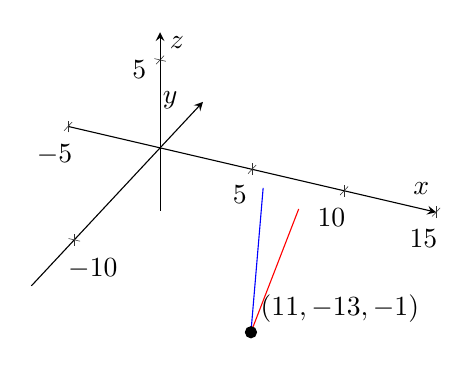
\begin{tikzpicture}
        \begin{axis}[axis equal,
                     axis lines=middle,
                     xlabel=$x$,
                     ylabel=$y$,
                     zlabel=$z$,
                     xmin=-5, xmax=15,
                     ymin=-15, ymax=5,
                     zmin=-2, zmax=5,
                     clip=false]
          % Define the two lines as parametric vectors
          \addplot3[blue, variable=\t, domain=0:-2] ({7-2*t},{-3+5*t},{1+t});
          \addplot3[red, variable=\s, domain=0:3] ({8+s},{-1-4*s},{-1});

          % Find the point of intersection
          \coordinate (A) at (axis cs:11,-13,-1);
          
          % Draw the point of intersection
          \filldraw [black] (A) circle (2pt);
          \node [above right] at (A) {$(11,-13,-1)$};
        \end{axis}
    \end{tikzpicture}}
\end{frame}
\subsection{Gaussian Elimination}
\frame{\subsectionpage}
\begin{frame}{Gaussian Elimination}
    \textbf{What is Gaussian Elimination?}
    \begin{itemize}
        \item<2->{A method of solving a system of linear equations.}
        \item<3->{A method of reducing a system of equations to a triangular matrix.}
        \item<4->{A method of reducing a system of equations to a diagonal matrix.}
    \end{itemize}
\end{frame}
\begin{frame}{Gaussian Elimination}
    \textbf{Why is Gaussian Elimination useful for this objective?}
    \begin{itemize}
        \item<2->{Currently, we've only been dealing with the intersections of 3-dimensional vectors.}
        \item<3->{But what if we wanted to find the intersection of an \begingroup\color{orange}{\bm{$n$}}\endgroup -dimensional vector \begingroup\color{orange}{\bm{$\vec{v}$}}\endgroup \ such that \begingroup\color{orange}{\bm{$\vec{v}$}} \endgroup \ is spanned over all real numbers (\begingroup\color{orange}{\bm{$\vec{v} \in \mathbb{R}^n$}}\endgroup )?}
        \item<4->{Alternatively, what if we wanted to solve for the intersection of more than two vectors?}
        \item<5->{This would make our system of equations quite complicated, and we wouldn't be able to solve it by hand... that is, unless we use Gaussian Elimination.}
    \end{itemize}
\end{frame}
\begin{frame}
    \frametitle{Reduced row echelon form (RREF)}
    \underline{Definition:} To be in RREF, a matrix $A$ must satisfy the following 4 properties (if it satisfies just the first 3 properties, it is in REF):
    \begin{enumerate}[1.]
        \item<2->{If a row does not have only zeros, then its first nonzero number is a $1$. We call this a {\em leading $1$}.}
        \item<3->{The rows that contain only zeros (if there are any) are at the bottom of the matrix.}
        \item<4->{In any consecutive rows that do not have only zeros, the leading $1$ in the lower row is farther right than the leading $1$ in the row above.}
        \item<5->{Each column that contains a leading $1$ has zeros everywhere else in that column.}
    \end{enumerate}
\end{frame}
\begin{frame}{Write out the augmented matrix}
    A system of linear equation is generally of the form
    \begin{equation}
        \label{e.linear}
        A \, \x = \b \,,
    \end{equation}
    where $A \in M(n \times m)$ and $\b \in \R^n$ are given, and $\x=(x_1, \dots, x_m)^T$ is the vector of unknowns.  For example, the system
    \begin{align*}
        x_2 + 2 \, x_3 - x_4 & = 1 \\
        x_1 + x_3 + x_4 & = 4 \\
        -x_1 + x_2 - x_4 & = 2 \\
        2 \, x_2 + 3 \, x_3 - x_4 & = 7
    \end{align*}
    can be written in the form \eqref{e.linear} with...
\end{frame}
\begin{frame}{Write out the augmented matrix}
    \begin{equation*}
        A = 
        \begin{pmatrix}
        0 & 1 & 2 & -1 \\
        1 & 0 & 1 & 1 \\
        -1 & 1 & 0 & -1 \\
        0 & 2 & 3 & -1
        \end{pmatrix} \,,
        \qquad \b =
        \begin{pmatrix}
        1 \\ 4 \\ 2 \\ 7 
        \end{pmatrix} \,.
      \end{equation*}
      \uncover<2>{Once you have the augmented matrix, you need to perform elementary row operations to get the matrix into RREF/REF. Then, you can solve for the unknowns.}
      \uncover<3>{However, I will not be going any more in depth into Gaussian Elimination becaue it is out of the scope for this presentation and I don't want to kill myself writing \LaTeX \ any further.}
\end{frame}
\subsection{Objective Summary}
\frame{\subsectionpage}
\begin{frame}{Objective Summary}
    \textbf{To find the point of intersection between two vectors:}
    \begin{itemize}
        \item<2->{Find the vector equations for each vector.}
        \item<3->{Set the two vectors equal to each other.}
        \item<4->{Solve for a parameter.}
        \item<5->{Substitute the parameter into one of the vector equations to find the point of intersection.}
    \end{itemize}
\end{frame}
    \addtocontents{toc}{\newpage}
    \section{Objective 26}
\subsection{}
\frame{\sectionpage}
\subsection{Terminology}
\frame{\subsectionpage}
\begin{frame}{Definitions}
    \begin{itemize}
        \item<1->{A \textcolor{orange}{\textbf{vector-valued equation}} is an equation that expresses a vector in terms of a parameter.}
        \item<2->{A \textcolor{orange}{\textbf{line}} is a straight path that extends infinitely in two directions.}
        \item<3->{\textcolor{orange}{\textbf{Three-dimensional space}} is the space in which three coordinates are needed to specify a point.}
    \end{itemize}
\end{frame}
\subsection{Objective Defined}
\frame{\subsectionpage}
\begin{frame}{What is Objective 26?}
    \begin{block}{Objective Definition}
        In this objective, you must be able to... \\
        \color{orange}{``Write the vector-valued equation of a line in three dimensions.``}
    \end{block}
\end{frame}
\begin{frame}{But what does that mean?}
    \begin{itemize}
        \item<1-2>{Well, in baby terms...}
        \begin{itemize}
            \item<2>{We want to write an equation that tells us where a line is in 3D space.}
        \end{itemize}
    \end{itemize}
\end{frame}
\subsection{\textit{Modus Operandi}}
\frame{\subsectionpage}
\begin{frame}{Formula}
    \begin{block}{Formula}
        A line in three dimensions can be defined by a vector-valued equation
        \begin{align*}
            \vec{r}(t) = r_0 + t \vec{v}
        \end{align*}
    \end{block}
\end{frame}
\begin{frame}{Formula}
    \begin{block}{Formula (cont.)}
        Where:
        \begin{itemize}
            \item<2->{\begingroup\color{orange}{\bm{$\vec{r}(t)$}}\endgroup \ is the vector-valued equation of the line.}
            \item<3->{\begingroup\color{orange}{\bm{$r_0$}}\endgroup \ is the starting point of the line.}
            \item<4->{\begingroup\color{orange}{\bm{$t$}}\endgroup \ is the parameter used to determine the position of any point on the line.}
            \item<5>{\begingroup\color{orange}{\bm{$\vec{v}$}}\endgroup \ is the direction vector of the line.}
        \end{itemize}
    \end{block}
\end{frame}
\subsection{Explanation}
\frame{\subsectionpage}
\begin{frame}{Explanation}
    \uncover<1->{\textbf{So, what was all of that?}}
    \begin{itemize}
        \item<2->{By using a vector-valued equation with a parameter \begingroup\color{orange}{\bm{$t$}}\endgroup , we can represent any point on the line by substituting different values of \begingroup\color{orange}{\bm{$t$}}\endgroup \ into the equation.}
        \item<3->{The direction vector \begingroup\color{orange}{\bm{$\vec{v}$}}\endgroup \ determines the slope of the line, and the starting point \begingroup\color{orange}{\bm{$a$}}\endgroup \ determines where the line begins.}
    \end{itemize}
\end{frame}
\subsection{Example}
\frame{\subsectionpage}
\begin{frame}{Example}
    \textbf{Example}
    \begin{block}{Problem}
        \textbf{What is the vector equation of a line that passes through the points (2, 4, -3) and (4, 1, 5)?}
    \end{block}
\end{frame}
\begin{frame}{Example}
    \textbf{First, we need to find the direction vector. Let point (2, 4, -3) equal \begingroup\color{orange}{\bm{$A$}}\endgroup \ and point   equal \begingroup\color{orange}{\bm{$B$}}\endgroup :}
    \begin{align*}
        \uncover<2->{\vec{AB} = \langle 4-2, 1-4, 5-(-3) \rangle} \\
        \uncover<3->{= \langle 2, -3, 8 \rangle}
    \end{align*}
\end{frame}
\begin{frame}{Example}
    \textbf{Now, we need to get the starting point, or \begingroup\color{orange}{\bm{$r_0$}}\endgroup .} \\
    \uncover<2->{\textbf{Since we chose \begingroup\color{orange}{\bm{$A$}}\endgroup \ to be the initial point of \begingroup\color{orange}{\bm{$\vec{AB}$}}\endgroup , we can just use the coordinates of  \begingroup\color{orange}{\bm{$A$}}\endgroup \ as  \begingroup\color{orange}{\bm{$r_0$}}\endgroup .}}
    \begin{align*}
        \uncover<3->{r_0 = (2, 4, -3)}
    \end{align*}
\end{frame}
\begin{frame}{Example}
    \textbf{Now, we can put it all together:}
    \begin{align*}
        \uncover<2->{r = r_0 + t \vec{v}} \\
        \uncover<3->{r_0 = (2, 4, -3)} \\
        \uncover<4->{\vec{v} = \vec{AB} = \langle 2, -3, 8 \rangle} \\
        \uncover<5->{r = \langle 1+3t, 3-2t, -2+7t \rangle} \\
    \end{align*}
    \uncover<6->{\textbf{We could have also done it in the opposite direction as long as we set \begingroup\color{orange}{\bm{$r_0$}}\endgroup \ to be \begingroup\color{orange}{\bm{$B$}}\endgroup \ and set \begingroup\color{orange}{\bm{$v$}}\endgroup \ to be \begingroup\color{orange}{\bm{$\vec{BA}$}}\endgroup.}}
\end{frame}
\begin{frame}{Example}
    \textbf{A substandard visual}
    \uncover<2->{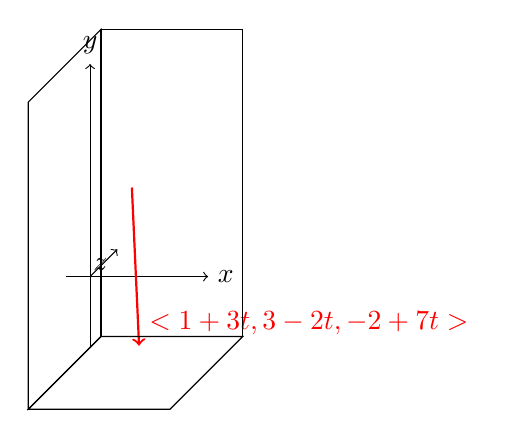
\begin{tikzpicture}[scale=0.3]
        % Set axis limits
        \draw[->] (-1,0) -- (5,0) node[right] {$x$};
        \draw[->] (0,-3) -- (0,9) node[above] {$y$};
        \draw[->] (0,0) -- (0,0,-3) node[below left] {$z$};
        
        % Plot vector equation
        \draw[red,thick,->] (1,3,-2) -- (4,-1,5) node[above right] {$<1+3t, 3-2t, -2+7t>$};
        
        % Adjust axis limits
        \pgfmathsetmacro{\xmax}{5.5}
        \pgfmathsetmacro{\ymax}{9.5}
        \pgfmathsetmacro{\zmax}{5.5}
        \pgfmathsetmacro{\xmin}{-0.5}
        \pgfmathsetmacro{\ymin}{-3.5}
        \pgfmathsetmacro{\zmin}{-2.5}
        \draw (\xmin,\ymin,\zmin) -- (\xmax,\ymin,\zmin) -- (\xmax,\ymax,\zmin) -- (\xmin,\ymax,\zmin) -- cycle;
        \draw (\xmin,\ymin,\zmin) -- (\xmin,\ymin,\zmax) -- (\xmin,\ymax,\zmax) -- (\xmin,\ymax,\zmin) -- cycle;
        \draw (\xmin,\ymin,\zmin) -- (\xmin,\ymin,\zmax) -- (\xmax,\ymin,\zmax) -- (\xmax,\ymin,\zmin) -- cycle;
        
        \end{tikzpicture}}
\end{frame}
\subsection{Objective Summary}
\frame{\subsectionpage}
\begin{frame}{Objective Summary}
    \textbf{To write the vector-valued equation of a line in three dimensions:}
    \begin{itemize}
        \item<2->{Find the direction vector.}
        \item<3->{Find the starting point.}
        \item<4->{Write the vector-valued equation.}
    \end{itemize}
    \uncover<5->{\textbf{Remember:} \textit{The direction vector determines the slope of the line, and the starting point determines where the line begins.}}
\end{frame}


    \section{Acknowledgments}
    \frame{\sectionpage}
        \begin{frame}{Acknowledgments}
            \textcolor{orange}{The authors are sincerely grateful to their teacher Mr. Cook for his superior seminars and notes about these objectives in his Advanced Calculus II class.}
        \end{frame}

    \begin{frame}{}
        \centering
            \Huge\bfseries
        \textcolor{orange}{Any questions?}
    \end{frame}
\end{document}